%----------------------------------------------------------------
%
%  File    :  project.tex
%
%  Author  :  Keith Andrews, IICM, TU Graz, Austria
%
%  Created :  24 Mar 2010
%
%  Changed :  06 Dec 2016
%
%----------------------------------------------------------------


\documentclass[11pt,onecolumn,twoside]{report}

\usepackage[          % set page and margin sizes
  a4paper,
  twoside,
  top=5mm,
  bottom=10mm,
  inner=15mm,
  outer=15mm,
  bindingoffset=10mm,
  head=10mm,
  foot=10mm,
  headsep=15mm,
  footskip=15mm,
  includeheadfoot,
]{geometry}
% A4 is 210 x 297 mm



\usepackage{txfonts}            % new times fonts
\usepackage{relsize}            % relative font sizes \smaller \larger
\usepackage{float}              % H for float placement
\usepackage{setspace}           % line spacing

\usepackage[T1]{fontenc}        % 8-bit output chars (must be before inputenx)
\usepackage[utf8]{inputenx}     % input char encoding

\usepackage{textcomp}           % symbols such as \texttimes and \texteuro
\usepackage{latexsym}

\usepackage{xspace}
\usepackage{etoolbox}           % for \newrobustcmd
\usepackage{makecmds}           % for \makecommand


\usepackage[english,austrian,british]{babel}


\usepackage[bf,sf]{titlesec}



\setlength{\textfloatsep}{10mm plus 2mm minus 1mm}
\setlength{\floatsep}{10mm plus 2mm minus 1mm}
\setlength{\intextsep}{10mm plus 2mm minus 1mm}

\setlength{\dbltextfloatsep}{10mm plus 2mm minus 1mm}
\setlength{\dblfloatsep}{10mm plus 2mm minus 1mm}

\setlength{\abovecaptionskip}{4mm plus 2mm minus 1mm}
\setlength{\belowcaptionskip}{0mm}




% use caption and subfig (caption2 and subfigure are now obsolete)

\usepackage[
  position=bottom,
  margin=1cm,
  font=small,
  labelfont={bf,sf},
  format=hang,
  indention=0mm,
]{caption}
% ]{caption,subfig}

\usepackage{subcaption}

\captionsetup[subfigure]{
  margin=0pt,
  parskip=0pt,
  hangindent=0pt,
  indention=0pt,
  singlelinecheck=true,
}




% fancyhdr to make nice headers and footers
% and deal with long chapter names

\usepackage{fancyhdr}         % headers and footers
\pagestyle{fancy}             % must call to set defaults before redefining

\renewcommand{\chaptermark}[1]{%
  \markboth{\thechapter.\ #1}{}
}
\renewcommand{\sectionmark}[1]{%
  \markright{\thesection.\ #1}
}
\renewcommand{\headrulewidth}{0mm}
\renewcommand{\footrulewidth}{0mm}
\newcommand{\headlook}{\sffamily}
\fancyhf{}
\fancyhead[LE,RO]{\thepage}
\fancyhead[LO]{%
\parbox[t]{0.8\textwidth}{\headlook\nouppercase{\rightmark}}
}
\fancyhead[RE]{%
\parbox[t]{0.8\textwidth}{\raggedleft\headlook\nouppercase{\leftmark}}
}


%\fancypagestyle{plain}{%   redefine plain style, but doesn't work
%  \fancyhf{}    % clear all header and footer fields
%  \fancyfoot[C]{\headlook \thepage} % except the center
%  \renewcommand{\headrulewidth}{0pt}
%  \renewcommand{\footrulewidth}{0pt}
%}



\usepackage{xcolor}
\definecolor{darkgreen}{rgb}{0.0,0.2,0.0}
\definecolor{darkblue}{rgb}{0.0,0.0,0.2}
\definecolor{darkred}{rgb}{0.2,0.0,0.0}
\definecolor{verylightgrey}{gray}{0.95}
\definecolor{lightgrey}{gray}{0.9}
\definecolor{black}{gray}{0.0}


\usepackage{tabularx}


\usepackage{listings}                 % for listings of source code
\usepackage{calc}                     % for calulation below

\makeatletter
\newlength{\numwidth}%
\setlength{\numwidth}{\widthof{\normalfont{\lst@numberstyle{99}}}}% Up to 2-digit (99) line numbers
\def\lst@PlaceNumber{%
  \makebox[\numwidth+1em][l]{%
    \makebox[\numwidth][r]{\normalfont\lst@numberstyle{\thelstnumber}}%
  }%
}
\makeatother

\lstset{                              % set parameters for listings
  floatplacement=tp,                  % default float placement
  numberbychapter,
  inputencoding=utf8,
  language=,                          % empty = plain text
  basicstyle=\small\ttfamily,
  tabsize=2,
  xleftmargin=1cm,
  xrightmargin=1cm,
  frame=none,
  framexleftmargin=0mm,
  rulesepcolor=\color{verylightgrey},
  numbers=none,
  numberstyle=\scriptsize,
  numbersep=2ex,
  breaklines,
  showtabs=false,
  showspaces=false,
  showstringspaces=false,
  keywordstyle=\bfseries,
  identifierstyle=,
  stringstyle=,
  captionpos=b,
  abovecaptionskip=\abovecaptionskip,
  belowcaptionskip=\belowcaptionskip,
  aboveskip=\floatsep,
  belowskip=\floatsep,
  extendedchars=true,
  literate=%
    {©}{{\textcopyright}}1
    {€}{{\texteuro}}1
    {Ö}{{\"O}}1
    {Ä}{{\"A}}1
    {Ü}{{\"U}}1
    {ß}{{\ss}}1
    {ö}{{\"o}}1
    {ä}{{\"a}}1
    {ü}{{\"u}}1,       % map some utf8 chars to replacements
}


\lstdefinelanguage{biblatex}   % based on biblatex v 2.7a from 2013-07-14
{
  keywords={%
    @article,@book,@mvbook,@inbook,@bookinbook,@suppbook,%
    @booklet,@collection,@mvcollection,@incollection,@suppcollection,%
    @manual,@misc,@online,@patent,@periodical,@suppperiodical,%
    @proceedings,@mvproceedings,@inproceedings,@reference,@mvreference,%
    @inreference,@report,@set,@thesis,@unpublished,@xdata,%
    @conference,@electronic,@mastersthesis,@phdthesis,@techreport,@www,%
    @artwork,@audio,@bibnote,@commentary,@image,@jurisdiction,@legislation,%
    @legal,@letter,@movie,@music,@performance,@review,@software,%
    @standard,@video%
  },
  comment=[l][\itshape]{@comment},
  sensitive=false,
}


\usepackage[short]{datetime}   % load datetime *after* babel, requires fmtcount
% \newdateformat{britdate}{%
% \ordinaldate{\THEDAY} \,\monthname[\THEMONTH] \THEYEAR
% }
\newdateformat{keithdate}{%
\twodigit{\THEDAY}~\shortmonthname[\THEMONTH]~\THEYEAR
}


\usepackage[hyphens,obeyspaces]{url}
\def\UrlFont{\smaller\ttfamily}



\usepackage[
  autostyle,
  english=british,
  threshold=0,
  thresholdtype=lines,
]{csquotes}
\renewcommand{\mkcitation}[1]{\space#1}

\newenvironment*{smallquote}          % smaller text within a block quote
  {\quote\smaller}
  {\endquote}
\SetBlockEnvironment{smallquote}

% put quotation marks around block quotes
% \renewenvironment{quoteblock}{\openautoquote}{\closeautoquote}

% I prefer double quotes as outer
\DeclareQuoteStyle[keithbritish]{british}%  [variant]{style}
  {\textquotedblleft}%                      opening outer mark
  {\textquotedblright}%                     closing outer mark
  [0.05em]%
  {\textquoteleft}%                         opening inner mark
  {\textquoteright}%                        closing inner mark

\setquotestyle[keithbritish]{british}



\usepackage[
  backend=biber,
  bibstyle=authoryear-ka,
  citestyle=authoryear-ka,
  sorting=nyt,
  useprefix,                   % van and von are part of second name
  mergedate=false,             % only for authoryear style
  dashed=false,                % only for authoryear style
  abbreviate=false,
  maxcitenames=2,              % if more than two authors, then use et al
  mincitenames=1,              % if exceeds 2 authors, then use 2
  maxbibnames=99,              % print all authors in biblio
  uniquename=init,
  hyperref=true,
  backref=true,
  backrefstyle=two,
  natbib=true,
  sortlocale=en,
]{biblatex}



% set for csquotes, but \autocite only available
% after biblatex is loaded
\SetCiteCommand{\autocite}    % or maybe \parencite

% more space between entries in bib
\setlength\bibitemsep{1.5\itemsep}


% remove URL: from in front of URLs
\DeclareFieldFormat{url}{\url{#1}}
\DeclareFieldFormat{doi}{\doi{#1}}
\DeclareFieldFormat{isbn}{\isbn{#1}}
\DeclareFieldFormat{issn}{\issn{#1}}

% suppress urldate field
\DeclareSourcemap{
  \maps[datatype=bibtex]{
    \map{
      \step[fieldset=urldate, null]
    }
  }
}

% for article titles
\DeclareFieldFormat{title:article}{\emph{#1}\midsentence}

\DefineBibliographyStrings{british}{%
  january          = {Jan},
  february         = {Feb},
  march            = {Mar},
  april            = {Apr},
  may              = {May},
  june             = {Jun},
  july             = {Jul},
  august           = {Aug},
  september        = {Sep},
  october          = {Oct},
  november         = {Nov},
  december         = {Dec},
}



% \bibliography{kandrews,latex,writing,inm-plag}

%\addbibresource{writing.bib}
%\addbibresource{latex.bib}
%\addbibresource{kandrews.bib}
%\addbibresource{ivis.bib}
\addbibresource{G5.bib}
\addbibresource{images/imgLocations.bib}
\addbibresource{listings/codeSource.bib}




\usepackage{ifpdf}

\ifpdf
  % pdflatex
  \usepackage[pdftex]{graphicx}
  \DeclareGraphicsExtensions{.pdf,.jpg,.png}
  \pdfcompresslevel=9
  \pdfpageheight=297mm
  \pdfpagewidth=210mm
  \usepackage[         % hyperref should be last package loaded
    unicode,
    pdftex,
    pdftitle={Animated rslidy: Responsive HTML5 Slide Decks},
    pdfsubject={},
    pdfauthor={Rok Kogovšek, Alexei Kruglov, Fernando Pulido Ruiz, and Helmut Zöhrer},
    pdfkeywords={project, IAWEB, animation, UI, web},
    bookmarks,
    bookmarksnumbered,
    linktocpage,
    colorlinks,
    linkcolor=darkred,
    anchorcolor=red,
    citecolor=darkgreen,
    urlcolor=darkblue,
    pdfview={FitH},
    pdfstartview={Fit},
    pdfpagemode=UseOutlines,       % open bookmarks in Acrobat
    plainpages=false,              % avoids duplicate page number problem
    pdfpagelabels,                 % avoids duplicate page number problem
    breaklinks=true,               % allow links exceeding a single line
  ]{hyperref}

\else
  % latex
  % should never have to run latex, since l2h now understands pdflatex .aux
  \usepackage[dvips]{graphicx}
  \usepackage[dvips]{hyperref}
  \DeclareGraphicsExtensions{.eps}
\fi





% \liintro list item intro is a style used when list items have an
% introduction phrase (say in italics) followed by a colon.
\newcommand{\liintro}[1]{\emph{#1}}


\newcommand{\imgcredit}[1]
{\smaller{}[#1]}



\newcommand{\copyrightACM}
{%
Copyright \copyright\ by the Association for Computing Machinery, Inc.%
}




\newcommand{\daymonthyear}[3]
{%
\twodigit{#1}\hspace{0.7ex}\nolinebreak[2]\shortmonthname[#2]\hspace{0.7ex}\nolinebreak[2]#3%
}


\newcommand{\monthyear}[2]
{%
\shortmonthname[#1]\hspace{0.7ex}\nolinebreak[2]#2%
}


\newcommand{\yearmonthday}[3]
{%
\twodigit{#3}\hspace{0.7ex}\nolinebreak[2]\shortmonthname[#2]\hspace{0.7ex}\nolinebreak[2]#1%
}


\newcommand{\yearmonth}[2]
{%
\shortmonthname[#2]\hspace{0.7ex}\nolinebreak[2]#1%
}



% link to Amazon or
% http://worldcatlibraries.org/wcpa/isbn/[ISBN number]

\newrobustcmd{\isbn}[1]
{%
{%
\ifpdf
{\smaller ISBN}
\href{http://www.amazon.com/exec/obidos/ASIN/#1/keithandrewshcic}{#1}%
\else
{\smaller ISBN}
#1%
\fi
}%
}



% ISSN
% http://www.bl.uk/services/bibliographic/issn.html
% 8 digits, should be printed xxxx-xxxx
% e.g. 0020-0190 is Information Processing Letters, Elsevier
%
% Lookup services:
% http://kmittlib.lib.kmutt.ac.th:81/search/i?SEARCH=0020-0190
% http://worldcatlibraries.org/wcpa/issn/0020-0190

\newrobustcmd{\issn}[1]
{%
{%
\ifpdf
{\smaller ISSN}
\href{http://worldcatlibraries.org/wcpa/issn/#1}{#1}%
\else
{\smaller ISSN}
#1%
\fi
}%
}



% DOIs  http://www.doi.org/  e.g.
% doi:10.1038/nature723
% http://dx.doi.org/10.1038/nature723

\newrobustcmd{\doi}[1]
{%
{%
\def\UrlFont{\rmfamily}
\ifpdf                                   % pdflatex
\href{http://dx.doi.org/#1}{doi:\protect\nolinkurl{#1}}%
\else                                    % latex
doi:\protect\nolinkurl{#1}%
\fi
}%
}





\newrobustcmd{\website}[1]
{%
\ifpdf                                  % pdflatex
\href{http://#1/}{\nolinkurl{#1}}%
\else                                   % latex
\nolinkurl{#1}%
\fi
}




\newcommand{\news}[1]
{%
\ifpdf
\href{news:#1}{\nolinkurl{#1}}
\else
\nolinkurl{#1}%
\fi
}








% based on url package
% define styles for class, file, and variable names
% which break nicely at line breaks

% make the macros robust so they work inside captions, etc

\newcommand{\ttname}{\begingroup \smaller\urlstyle{tt}\Url}
\newcommand{\rmname}{\begingroup \smaller\urlstyle{rm}\Url}
\newcommand{\sfname}{\begingroup \smaller\urlstyle{sf}\Url}


% cname is for class names
\newrobustcmd{\cname}[1]{\sfname{#1}}

% fname is for file names and directory names
\newrobustcmd{\fname}[1]{\ttname{#1}}

% vname is for variable names, domain names, email addresses
\newrobustcmd{\vname}[1]{\ttname{#1}}



% Euro symbol
\newcommand{\euro}{\texteuro\,}

% times symbol
\newcommand{\timessym}{\texttimes\,}

% approx symbol
\newcommand{\approxsym}{\ensuremath\approx\,}

% plusminus symbol
\newcommand{\plusminussym}{\textpm\,}

% not equal symbol
\newcommand{\neqsym}{\ensuremath{\neq\,}}

% rightarrow symbol
\newcommand{\rightarrowsym}{\ensuremath\rightarrow\,\,}




\newcommand{\TODO}[1]
{
{\textcolor{red}{[TODO: #1]}}
}



\newcommand{\fullh}{18cm}         % height of figures for 1 per page
\newcommand{\halfh}{9.5cm}        % height of figures for 2 per page
\newcommand{\thirdh}{6cm}         % height of figures for 3 per page


\tolerance=400 
  % makes some lines with lots of white space, but      
  % tends to prevent words from sticking out in the margin





\definecolor{lightgray}{rgb}{.9,.9,.9}
\definecolor{darkgray}{rgb}{.4,.4,.4}
\definecolor{purple}{rgb}{0.65, 0.12, 0.82}
\lstdefinelanguage{JavaScript}{
	keywords={break, case, catch, continue, debugger, default, delete, do, else, false, finally, for, function, if, in, instanceof, new, null, return, switch, this, throw, true, try, typeof, var, void, while, with},
	morecomment=[l]{//},
	morecomment=[s]{/*}{*/},
	morestring=[b]',
	morestring=[b]",
	ndkeywords={class, export, boolean, throw, implements, import, this},
	keywordstyle=\color{blue}\bfseries,
	ndkeywordstyle=\color{darkgray}\bfseries,
	identifierstyle=\color{black},
	commentstyle=\color{purple}\ttfamily,
	stringstyle=\color{red}\ttfamily,
	sensitive=true
}






\lstset{
	backgroundcolor=\color{lightgray},
	float=tp,
	xleftmargin=1cm,
	xrightmargin=1cm,
    framexleftmargin=1mm,
	extendedchars=true,
	basicstyle=\footnotesize\ttfamily,
	showstringspaces=false,
	showspaces=false,
	numbers=left,
	numberstyle=\footnotesize,
	numbersep=9pt,
	tabsize=2,
	breaklines=true,
	showtabs=false,
	captionpos=b
}



\begin{document}

\keithdate

\normalsize
\pagestyle{empty}         % for preliminary pages (no numbers shown)
\pagenumbering{Roman}     % for pdf labels




\begin{titlepage}

\begin{center}
{\Large \sffamily \bfseries Animated rSlidy \\ Responsive HTML5 Slide Decks}

\vspace{1cm}

% {\large\sffamily Keith Andrews}

{\large\sffamily Group 5}

\vspace{5mm}

{\large\sffamily Rok Kogovšek, Alexei Kruglov, Fernando Pulido Ruiz, and Helmut Zöhrer}

\vspace{1cm}

% Institute for Information Systems and Computer Media (IICM), \\
% Graz University of Technology \\
% A-8010 Graz, Austria \\[1cm]


{\large
706.041 Information Architecture and Web Usability WS 2016 \\
Graz University of Technology \\
A-8010 Graz, Austria  \\[1cm]
}

\vspace{1cm}

% {\large 22 Nov 2016}

{\large \today}


\end{center}



\vspace{2cm}

\begin{quote}
\begin{center}
{\large\sffamily\bfseries Abstract}
\end{center}

This project report tries to give insights into the implementation of refinements of the already existent presentation software \textit{rslidy} provided by Keith Andrews of TUG.. It includes direct comparisons of the initial and the new version(s) in terms of design and functionality. Not only this contrast, but also the particular ways of implementing certain new features are listed and discussed.The focus of the project was to make the already working version of the web slideshow application closer to well spread desktop solutions. This entitled improving the user interface to be more interactive, responsive and user friendly. A big focus of the project was on animation solutions.


\end{quote}

\vfill

\begin{center}
{\small\sffamily \copyright ~ Copyright 2017 by the author(s),
except as otherwise noted.}

\vspace{2mm}
{\footnotesize\sffamily This work is placed under a
Creative Commons Attribution 4.0 International
(\href{https://creativecommons.org/licenses/by/4.0/}{CC BY 4.0}) licence. It uses the LaTex template from "Writing a Survey Paper" by Keith Andrews, used under CC BY 4.0 / Desaturated from original
}
\end{center}

\end{titlepage}




\cleardoublepage
\pagestyle{plain}
\pagenumbering{roman}



{
\setlength{\parskip}{3pt plus 3pt minus 3pt}     % compact tables of contents
\tableofcontents
\addcontentsline{toc}{chapter}{Contents}

\cleardoublepage
\listoffigures
\addcontentsline{toc}{chapter}{List of Figures}

%\cleardoublepage
%\listoftables
%\addcontentsline{toc}{chapter}{List of Tables}

\cleardoublepage
\renewcommand{\lstlistlistingname}{List of Listings}
\lstlistoflistings
\addcontentsline{toc}{chapter}{List of Listings}
}

% define CSS source code coloring
\lstdefinelanguage{CSS} 
{
alsoletter={<>/.\#},
keywords={},
% CSS properties
keywords={ border,transform,origin,transition,duration,timing-function,animation,color,background,margin,padding,font,weight,display,position,top,left,right,bottom,list,style,size,white,space,min,width,opacity,height,delay, content,radius, stroke, fill, cx, cy,attributeName, attributeType, values, type, dur, repeatCount, viewBox, d},
% CSS rules
keywords=[2]{@keyframes},
% CSS selectors
keywords=[3]{hover,before,after, nth, child},
% HTML attributes
keywords=[4]{class, alt, id, role, href,
% calss names for linking it together with CSS
desiredName, spin, rotating, bar, loading, dots, move, pulz, delete, rot, docs, decks },
% HTML tags
keywords=[5]{
  >, />, <html>, , </html> ,
  % body
  <body>, </body>,
  % Divs
  div, </div, <div, </div>, <div></div>,
  % Paragraphs
  </p, <p, </p>,
  % scripts
  </script, <script,
  % navigation
  a, <a, </a>,
  nav, <nav>, </nav>,
  ul, <ul>, </ul>,
  li, <li>, </li>, <li><a, </a></li>,
  % More tags...
  <canvas, /canvas>, <svg, <rect, <animateTransform, </rect>, </svg>, <video, <source, <iframe, </iframe>, </video>, <image, </image>, <header, </header, <article, </article, <circle, <path, </path>
  },
  keywords=[6]{
    .hamburger, .paperNav, container, .inner,
    .topBotomBordersOut, .borderYtoX, .highlightTextOut, .circleLoader, .squareloader,
    .dotsLoader, .progressbarloader,.pulzLoader, \#svg, doc, deck, .container
  },
sensitive=false,
mathescape=true,
morecomment=[l]{//}, 
morecomment=[s]{/*}{*/},
morestring=[b][\color{darkred}]",
morestring=[b][\color{darkred}]',
% morecomment=[s][\color{darkred}]{\ .}{\ },
keywordstyle=\color{blue},
keywordstyle=[2]\color{brown},
keywordstyle=[3]\color{orange},
keywordstyle=[4]\color{violet},
keywordstyle=[5]\color{teal},
keywordstyle=[6]\color{darkred}
}

\cleardoublepage
\pagestyle{headings}        % for main pages
\pagenumbering{arabic}

\cleardoublepage
%----------------------------------------------------------------
%
%  File    :  survey-intro.tex
%
%  Author  :  Keith Andrews, IICM, TU Graz, Austria
% 
%  Created :  27 May 1993
% 
%  Changed :  06 Dec 2016
% 
%----------------------------------------------------------------


\chapter{Introduction}

\label{chap:Intro}

Our group was assigned with the task of refining the already existent presentation software \textit{rSlidy}. Therefore we first made some usability tests on our own in order to become familiar with the software and to find room for improvement. We interactively agreed with our instructor on features that needed implementation and those which would be nice to have, but not necessary.

The final submission comprises two versions of the new \textit{rSlidy}. One which is completely independent and one which uses two third party libraries. The independent one might not look as impressive in some scenarios, but is free of external code. The other version is arguably better design-wise, but relies on third party libraries, which was not in favor of the instructor. 

%HEre we tell we prepared a rSlidy only upgrade and a rSlidy supported by 3rd party software

% Fernando Pulido Ruiz
\cleardoublepage
%----------------------------------------------------------------
%
%  File    :  survey-intro.tex
%
%  Author  :  Keith Andrews, IICM, TU Graz, Austria
% 
%  Created :  27 May 1993
% 
%  Changed :  03 Feb 2017
% 
%----------------------------------------------------------------


\chapter{rSlidy}

\label{chap:rslidy}

Fernando use that pdfyou found to write as much as possible about the original \textit{rSlidy}. And what where the reasons that this upgrade project was started - basicly the faults of the original \textit{rSlidy}.

\section{History?} % (fold)
\label{sec:history}

% section history (end)

\section{Installation} % (fold)
\label{sec:installation}

% section installation (end)

\section{Animated upgrade} % (fold)
\label{sec:}

Why we went to upgrade,
how the new code install is,
That there are 2 versions

% section  (end)

% Helmut Zöhrer
\cleardoublepage
%----------------------------------------------------------------
%
%  File    :  survey-design.tex
%
%  Author  :  Keith Andrews, IICM, TU Graz, Austria
% 
%  Created :  27 May 1993
% 
%  Changed :  03 Feb 2017
% 
%----------------------------------------------------------------


\chapter{Changes of the Design}

\label{chap:design}

The design of rSlidy has undergone numerous major changes throughout our project. A comparison between the old and the new version is given in this chapter.

\section{The Status Bar}
The initial version of rSlidy was equipped with a permanent status bar, as shown in Figure \ref{fig:statusbarOLD}.

It has been modified in terms of design and functionality. The final appearance of the status bar is shown in  Figure \ref{fig:statusbarNEW}. The following individual changes have been made.

\begin{figure}[tp]
	\centering
	
\includegraphics[width = \textwidth]{images/status_bar_old.png}
	
	\caption[Original Status Bar]{
		Design of rSlidy's original status bar.
		\imgcredit{Screenshot taken by the authors of this survey.}
	}
	\label{fig:statusbarOLD}
\end{figure}

\begin{figure}[tp]
	\centering
	\includegraphics[width = \textwidth]{images/status_bar_NEW.png}
	
	\caption[Modified Status Bar]{
		Design of rSlidy's modified status bar.
		\imgcredit{Screenshot taken by the authors of this survey.}
	}
	\label{fig:statusbarNEW}
\end{figure}


\subsection{Progress Bar}
A simple blue progress bar has been added on top of the status bar. Its purpose is to give some visual feedback about the current progress within a presentation. Its implementation is fairly simple.

A progress bar container was added at the desired position whose width property is changed on each slide change (see Listing \ref{list:progressbar}).


\begin{lstlisting}[
language=JavaScript,
label=list:progressbar,
caption={[Progress Bar Width Adaptation] Adapting width of the progress bar container for authentic visual feedback %
\imgcredit{The 
code example is based 
on the users' implementation.}
}
]
Rslidy.prototype.showSlide = function (slide_index) {
	// ...
	var progress_bar = document.getElementById("progress-bar");
	progress_bar.style.width =
				'calc(100%*' + (slide_index + 1) / this.num_slides + ')';
	// ...
}
\end{lstlisting}

\subsection{Rearrangement / Extension of the Navigation Elements}
We found it simply more intuitive to have the input field for jumping to a specific slide in the middle of the forward / backward buttons.

Apart from this, functionalities to jump to the first respectively the last slide have been added. These two starightforward implementations can be seen in Listing \ref{list:firstlastslide}.

\begin{minipage}{\linewidth}
\begin{lstlisting}[
language=JavaScript,
label=list:firstlastslide,
caption={[First / Last Slide Buttons Implementation] Implementation of the buttons for jumping to the first / last slide%
\imgcredit{The 
code example is based 
on the users' implementation.}
}
]
document.getElementById("status-bar-nav-button-first")
	.addEventListener('click', function ()
	{
		this.showSlide(0);
	}.bind(this));
document.getElementById("status-bar-nav-button-last")
	.addEventListener('click', function ()
	{
		this.showSlide(this.num_slides - 1);
	}.bind(this));
\end{lstlisting}
\end{minipage}



\subsection{Pin Functionality}
In opposition to the original rSlidy status bar, the new one features pinning / unpinning. The pinned status bar works the same as the old one. The unpinned status bar disappears when not hovering over it. When the mouse is not close to the bottom of the document, only the progress bar is visible in the unpinned mode. Two subtle triangles have been added to the unpinned status bar which are meant to function as little indicators for the actual bar. This implementation may not be the most elegant one, because it is relying on the title of the button to work properly. Some simple boolean variable which describes whether the bar is pinned or not may be a more robust solution. Still, this (see Listing \ref{list:pin_unpin}) is what we came up with and it works fine as long as the title tag of the pin button in the rslidy.js file is either "Pin the status bar" or "Unpin the status bar" (depending on whether the user wants the bar to be pinned or not by default).


\begin{minipage}{\linewidth}
\begin{lstlisting}[
language=JavaScript,
label=list:pin_unpin,
caption={[Pin / Unpin Implementation] Implementation of the buttons for pinning / unpinning the status bar %
\imgcredit{The 
code example is based 
on the users' implementation.}
}
]
Rslidy.prototype.pinToggleClicked = function (close_only) {
	var pin_button = document.getElementById("status-bar-pin-button");
	var status_bar = document.getElementById("status-bar-content");
	var indicator_left = document.getElementById("progress-bar-indicator-left");
	var indicator_right = document.getElementById("progress-bar-indicator-right");

	if (pin_button.title == "Pin the status bar")
	{
		pin_button.title = "Unpin the status bar";
		status_bar.style = "transform: translateY(0);";
		pin_button.style.WebkitTransition = 'opacity 0.3s';
		pin_button.style.MozTransition = 'opacity 0.3s';
		pin_button.style.opacity = 0.5;
		indicator_left.style.visibility = "hidden";
		indicator_right.style.visibility = "hidden";
	}
	else
	{			
		pin_button.title = "Pin the status bar";
		status_bar.removeAttribute('style');
		pin_button.style.opacity = 1;
		indicator_left.style.visibility = "visible";
		indicator_right.style.visibility = "visible";
	}
};
\end{lstlisting}
\end{minipage}

\subsection{Buttons animations}
Similar to an animated hamburger icon, which changes its shape on click, the buttons within the status bar of rSlidy are animated now as well. Listing \ref{list:buttonflip} shows how the animated flip was created. These style changes and the button's text changed to an "X" lead to a simple and intuitive animation of a button which turns around to change its functionality. 

\begin{minipage}{\linewidth}
	\begin{lstlisting}[
	language=CSS,
	label=list:buttonflip,
	caption={[Flip Button Animation] Implementation of the animation of the buttons in the status bar %
	\imgcredit{The 
	code example is based 
	on the users' implementation.}
	}
	]
#button-overview, #button-toc, #button-menu{ 
	animation-duration: 0.3s; 
	animation-timing-function: ease-in-out;
	animation-fill-mode: forwards;
	animation-name: flip2Face;
}

#button-overview.clicked, #button-toc.clicked, #button-menu.clicked{
	animation-name: flip2Back; 
	transform: rotateY(180);
}
	\end{lstlisting}
\end{minipage}






\section{The Menu}
The menu has been modernized and harmonized as seen in a direct comparison of Figure \ref{fig:menuOLD} and Figure \ref{fig:menuNEW}.

\begin{figure}[tp]
	\centering
	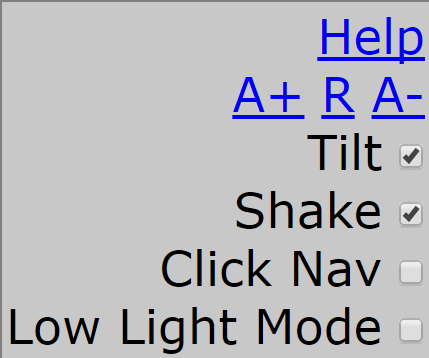
\includegraphics[width = .4\textwidth]{images/menu_old.png}
	
	\caption[Original Menu]{
		Design of rSlidy's original menu.
		\imgcredit{Screenshot taken by the authors of this survey.}
	}
	\label{fig:menuOLD}
\end{figure}

\begin{figure}[tp]
	\centering
	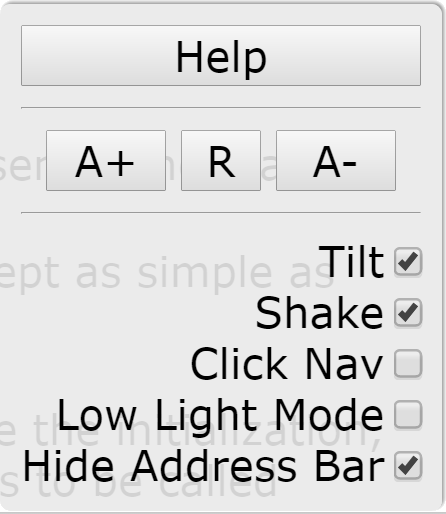
\includegraphics[width = .4\textwidth]{images/menu_new.png}
	
	\caption[Modified Menu]{
		Design of rSlidy's modified menu.
		\imgcredit{Screenshot taken by the authors of this survey.}
	}
	\label{fig:menuNEW}
\end{figure}

Implementation-wise these changes were mostly straightforward:
\begin{itemize}
	\item Partial transparency has been added to the menu. The actual document thus slightly shines through the menu.
	\item The corners have been corners in order to get a smoother look in general.
	\item Shadow effects have been added to the edges of the menu in order to get a very basic 3D-effect.
	\item Harmonization has taken place. All links were exchanged with buttons. This means more consistency in the design altogether. 
	\item One more checkbox has been added. It allows the user to switch between a version which, as usual, shows the address of a link on hover and a version which suppresses that standard function by removing the "href" property from all initial links.
\end{itemize}


\section{The Help Information}
This information, which can be opened from the menu, used to be a usual alert box. Due to the instructor's wish to have no third party libraries included, there are two versions of our implementation for the new help popup.

The initially intended version is based on a library called "sweetalert" (\url{https://limonte.github.io/sweetalert2/}). It allows animated popup messages with focusing on the actual text. The advantage of this way of implementation is the the polished design while having to rely on a third party library. 

The revised version simply opens a new tab to display the help message. This does not look as sophisticated as the other version, but still works fine and is an independent way of solving the popup problem.


% Alexei Kruglov
%----------------------------------------------------------------
%
%  File    :  survey-images.tex
%
%  Author  :  Keith Andrews, IICM, TU Graz, Austria
% 
%  Created :  27 May 1993
% 
%  Changed :  03 Feb 2017
% 
%----------------------------------------------------------------


\chapter{Image Magnification}

\label{chap:images}

In this part of the project we have focused on presentation of images. We have 
added a zoom feature, which opens the clicked picture in a new window or in the 
enhanced version in a pop-up. The implementation works on different picture 
formats, of which we tested svg, jpeg, gif and png. Our enhancements give users 
a better opportunity to see detailed parts of the selected image, by fitting it 
to the width of the screen, while supporting zooming for smaller details or 
prefered size readjustment. Since zooming is involved and screen space is 
limited, we solve the overflow problem with scroll bars.

\begin{figure}[hp]
\centering

\subcaptionbox[Original Presentation Image Size]{%
Size of image set by the presentation creator.%
  
    \label{subfig:realy_img}%
}
[%
    0.44\hsize % width of caption
]%
{%
    \includegraphics[keepaspectratio,width=0.45\hsize]%
    {images/image1.png}%
}%
\hspace{0.05\hsize} % seperation
\subcaptionbox[Image Zoom For Detail] {%
   Zoomed-in part of same image.%
    \label{subfig:zoomed_img}%
}
[%
    0.44\hsize % width of caption
]%
{%
    \includegraphics[keepaspectratio,width=0.45\hsize]%
    {images/image2.png}%
}%
\caption[]{A SVG image inside the presentation before and after the 
magnification click.
\imgcredit{Screenshots taken by the authors of this report, while the original 
image is from a provided presentation \citep{keithDataVis}.
\label{fig:popup}
}}

\end{figure}

On click the selected image opens in a new tab or in the enhanced version in a 
pop-up window. While the complex pop-up function is provided by a 3rd party 
solution, the simplier new tab opening is done by supplying HTML content 
through JavaScript's document.write function on a new blank document. The 
provided content includes the page layout, buttons, the magnified picture, and 
JavaScript, which is needed for image resizing. To simplify the JavaScript 
inclusion, a seperate function is written, which is then converted to tex 
through the String function.

\begin{figure}[tp]
\centering

\includegraphics[keepaspectratio,scale=0.5]{images/button.png}

\caption[Image Magnification Controls]{
The magnification control bar next to the zooming buttons includes an updatable 
label, to report the current zoom in regards to original image size. 
\imgcredit{Screenshot taken by the authors of this report.}

}
\label{fig:Buttons}
\end{figure}

\newpage

In either the popup or tab window we can zoom it for +-10\%, +-100\%, and 
+-1000\% by pressing the provided buttons. Alternatively with keyboard or mouse 
support, we can also zoom it with +/- keyboard buttons or CTRL plus mouse 
scrolling event by a the default step of 10. To fit it back into the default 
size, where zoom is 100\%, we can do it by pressing keyboard button 0.

\begin{lstlisting}[
language=JavaScript,
label=openImgCode,
caption={[Image Magnification Initialization]%
Implementation of image detection and click event binding of content push. The 
called function is for the tab solution, while the pop-up solution seperates 
the control bar in the 3rd party sweetalert function call for layout 
improvement.
}
]
	  // Input listeners
		var images = document.getElementsByTagName("img");
		var images  = content_section.getElementsByTagName("img");

		for (var i=0, len=images.length, img; i<len; i++) {
		  img = images[i];
		  img.addEventListener("click", function() {
			openImageTab(this.src);
		  });
		}
	};
}

function openImageTab(imgSrc) {
	var newWindow = window.open();
	
	var htmlCode ="<head><title>rSlidy Image View</title><link 
rel='stylesheet' href='css/reset.css'><link rel='stylesheet' 
href='css/normalise.css'>" +
			"<link rel='stylesheet' href='css/rslidy.css'><link 
rel='stylesheet' href='css/slides-default.css'></head>" +
			"<body><div class='slide 
imageAlert'><h1><button>-1000\%</button><button>-100\%</button><button>-10\%</bu
tton>Zoom at <span 
id='zoomNumber'>100</span>\%<button>+10\%</button><button>+100\%</button><button
>+1000\%</button></h1>" +
			"<div><img id='zoomedImg' src='"+ imgSrc + 
"'></div></div>"+
			"<script type='text/javascript'>" + 
String(openImageTabListeners) + "; openImageTabListeners();</script></body>";
	newWindow.document.write(htmlCode);
}
\end{lstlisting}

\newpage

\begin{lstlisting}[
language=JavaScript,
label=imgControls,
caption={[Image Magnification Controls]%
	The control functions for all events are same for both rSlidy versions.
}
]
	
	window.addEventListener('keypress', function (e) {
		if (e.key == '+' || e.key == '-' || e.key == '0') {
			var zoom = parseInt(titleElement.innerHTML);
			if(e.key == '+'){
				zoom = zoom + 10;
			}
			else if(e.key == '-')
			{
				zoom = zoom - 10;
			}
			else{
				zoom = 100;
			}
			if(zoom > 0){
				img.style.height = zoom * heightPer + "px";
				img.style.width = zoom * widthPer + "px";
				titleElement.innerHTML = zoom;
			}
		}
	}, false);

	var isCtrl = false;
	window.addEventListener('keydown', function (e) {
		if (e.which === 17) {
            isCtrl = true;
        }
    }, false);
	window.addEventListener('keyup', function (e) {
		if (e.which === 17) {
            isCtrl = false;
        }
    }, false);

	window.addEventListener("mousewheel", function (e) {
		if(isCtrl){
			var delta = Math.max(-1, Math.min(1, e.wheelDelta));
			var zoom = parseInt(titleElement.innerHTML);
			if(delta > 0){
				zoom = zoom + 10;
			}
			else if(delta < 0)
			{
				zoom = zoom - 10;
			}
			if(zoom > 0){
				img.style.height = zoom * heightPer + "px";
				img.style.width = zoom * widthPer + "px";
				titleElement.innerHTML = zoom;
			}
		}
	}, false);
}
\end{lstlisting}

% Rok Kogovšek
\cleardoublepage
%----------------------------------------------------------------
%
%  File    :  survey-animation.tex
%
%  Author  :  Keith Andrews, IICM, TU Graz, Austria
% 
%  Created :  27 May 1993
% 
%  Changed :  03 Feb 2017
% 
%----------------------------------------------------------------


\chapter{Animated Slideshow}

\label{chap:animated}

The biggest downside of the original \textit{rSlidy} when compared to 
alternative solutions, with focus on well spread desktop solutions, would be 
its static state. Namely the presentation flow achieved with the application 
was an immediate switch between states or slides. Even the user interface was 
behaving similarly in a state-switching way. In the design changes the effects 
of hiding elements with hover and transition CSS elements also include a better 
user experience. This follows the observations from the web animation survey 
\citet{WebAnime}, were the importance of animation for user experience was 
stressed out. With knowledge gathered from the mentioned survey we enhanced 
both the user interface as well the presentation flow by incorporating 
animation with CSS and JavaScript. For better overview, the animated old 
elements, that were already present in the original \textit{rSlidy}, have CSS 
added near the original class definitions, while the new concepts, sections 
\ref{sec:initialization} and \ref{sec:slide_transitions}, are defined in the 
new CSS file \textit{rslidy-animation.css}.

\section{Initialization Progress Animation} % (fold)
\label{sec:initialization}

A major problem with the original \textit{rSlidy} appeared when big slideshow 
files where loaded. Since at load all elements are hidden to be processed 
before presenting, for big files long unclear loading times appear. Such 
initialization is not friendly for the user and leaves a bad impression. 
Therefore we wanted to implement a simple loading animation, that would load 
quickly, represent the application and be entertaining for the short or long 
wait. We took inspiration from the simple but effective CSS implementation of a 
pulz loader\citep{WebAnime} and modified it to our needs. The result can be 
observed in figure \ref{fig:loading}, where we can see, that the modification 
leaves quite a different impression from the inspiration source. To achieve all 
desired properties of the loader we implemented an animation of the letters of 
\textit{rSlidy} form a mexican wave by jumping in delays. The design was kept 
simple also in colors, to be consistent with the color palate from the 
application.

\subsection{Rendering Waits for Break} % (fold)
\label{sub:rendering_waits_for_break}

A bit trickier was the inclusion of the the html code on loading time. When 
onLoad JavaScript is called, the browser rendering process is waiting for a 
stop, to draw anything. However the break happens once the function is closed, 
so a go-around with setTimeout function with 1ms delay is needed to call the 
initialization. The whole initialization is now done so, that firstly the 
loader HTML code is included in the body, afterwards the setTimeout is called, 
which calls a function that calls the init function from the Rslidy object to 
render the loader before the initialization. The loader is then hidden, when 
the same init function decides the current slide, which triggers the slide 
loading.

% subsection rendering_waits_for_break (end)


\begin{minipage}{\linewidth}
	\begin{lstlisting}[
	language=CSS,
	label=list:loaderCSS,
	caption={[Initialization Progress Animation] The designed loader simply 
has its inner divs that contain letters jump in the first 40\% of the animation 
time with 0.1s delays between jump starts.}
	]
#loader div{
	display: inline-block;
	padding: 0.2em;
	animation: jump-loading 1s ease-in-out infinite;
}

/*Change delay per child*/
#loader div:nth-child(1) {  animation-delay: 	0;	}
#loader div:nth-child(2) {  animation-delay: 0.1s;	}
#loader div:nth-child(3) {  animation-delay: 0.2s;	}
#loader div:nth-child(4) {  animation-delay: 0.3s;	}
#loader div:nth-child(5) {  animation-delay: 0.4s;	}
#loader div:nth-child(6) {  animation-delay: 0.5s;	}

@keyframes jump-loading {
	0%	{	transform: translate(0,		0);		}
	20% {	transform: translate(0, -1.5em);	}
	40% {	transform: translate(0,		0);		}
}
	\end{lstlisting}
\end{minipage}

\begin{figure}[tp]
	\centering
	
\includegraphics[width = .25\textwidth]{images/pulzLoad.png}
	
\includegraphics[width = .5\textwidth]{images/loading.png}	
	\caption[Loader]{
		Screenshot of the loading animations midway. On the left we see 
the inspirational pulz loader, while on the right we see the resulting 
rearrangement for \textit{rSlidy}.
		\imgcredit{Screenshot taken by the authors of this report.}
	}
	\label{fig:loading}
\end{figure}

% section initialization (end)

\section{Button Animation} % (fold)
\label{sec:button_animation}

Similar to an animated hamburger icon, which changes its shape on click, the 
buttons within the status bar of \textit{rSlidy} are animated now as well. 
Listing \ref{list:buttonflip} shows how the animated flip was created. These 
style changes and the button's text changed to an "X" lead to a simple and 
intuitive animation of a button which turns around to change its functionality. 
While the animation is done in CSS, the text change is done by the JavaScript 
setTimeout, to change the value halfway through the animation, when the text is 
not visible.
\begin{minipage}{\linewidth}
	\begin{lstlisting}[
	language=CSS,
	label=list:buttonflip,
	caption={[Flip Button Animation] Implementation of the animation of the 
buttons in the status bar
	}
	]
#button-overview, #button-toc, #button-menu{ 
	animation-duration: 0.3s; 
	animation-timing-function: ease-in-out;
	animation-fill-mode: forwards;
	animation-name: flip2Face;
}

#button-overview.clicked, #button-toc.clicked, #button-menu.clicked{
	animation-name: flip2Back; 
	transform: rotateY(180);
}
	\end{lstlisting}
\end{minipage}

\subsection{Same Element Animation Issue} % (fold)
\label{sub:same_element_animation_issue}

By having a direction and play animation property it seems that there is no 
need for two keyframe definitions, as in code snipplet \ref{list:buttonflip}. 
However getting it to work on same element is another issue. By researching 
forums, the main issue lies in the nature of CSS, overlaping properties from 
previous class, which seems to include counters. This becomes troublesome, when 
animation count is not infinite, like with button rotations example. While a 
simple transition would work if it was just a rotation, including a bit of 
scaling in the middle of the transformation to get a better effect, makes it 
impossible to solve with transitions. This issue became also a problem in 
section \ref{sec:slide_transitions}. The best pure CSS solution solution 
without adding additional HTML elements or doing JS animation was to actually 
write a reverse keframe copy and use that name in the needed class, which seems 
to reset the counter due animation initialization.

% subsection same_element_animation_issue (end)

% section button_animation (end)

\section{Hiding Elements} % (fold)
\label{sec:hiding_elements}

While hiding elements on hover elements by itself already raises the user 
experience, just by adding simple transition or animation CSS element we can 
direct the switch between states into a smooth way to enhance the user 
workflow. For better control we also used the Cubic Bezier function, with the 
values shown in figure \ref{fig:cubic-bezier}.

\begin{figure}[tp]
	\centering
	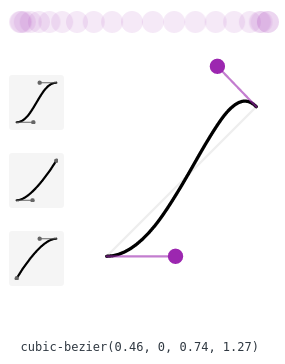
\includegraphics[width = .4\textwidth]{images/cubic-bezier.png}
	
	\caption[Cubic Bezier Function]{
		The values of the Cubic Bezier function used for smoother 
hiding of elements and its plot representation
		\imgcredit{Screenshot of the representation in Chrome Developer 
Tools taken by the authors of this report.}
	}
	\label{fig:cubic-bezier}
\end{figure}

% section hiding_elements (end)

\section{Preview Scrolling} % (fold)
\label{sec:preview_scrolling}

The Slides previous most of the time give you a nice preview of the slides. 
However depending on the amount of text or even the screen size due to using 
proportions for the thumbnails the preview may not be clear enough which slide 
it is due to the text overflow being hidden. Therefore we added a simple on 
hover animation of translating the thumbnail content by 20\% upwards. The only 
thing also to note was the choosing of the correct content to move. Namely 
moving the first child also moves the afixed click event, while further 
children had problems with z-indecies. Understanding the z-index property and 
the structure of your CSS code is the key for such situations. A great 
by-product of an on hover animation is that is a great indicator for the 
current mouse position, which the original \textit{rSlidy} on hover event only 
covered by slightly changing the color.

% section preview_scrolling (end)thumbnail
\newpage
\section{Slide Transitions} % (fold)
\label{sec:slide_transitions}

The last described animation was also the biggest contribution for a more 
dynamic presentetion flow. The goal was to include a simple way for the user to 
chose animated transitions between slides. To keep the previous version of 
immediate transitions also as an option of \textit{rSlidy}, we simply defined a 
body class \textit{animated}, on which all animated transition classes are 
referenced through.

First problem we faced was the original definition of \textit{hidden}, that 
uses display property set to none. This sets the the element not to be included 
in the render list of the browser, which however is required for animations to 
be applied. Since the display property is uncompatible with animation and the 
hiding of slides is the core of the application, we redefined the the 
\textit{hidden} for \textit{animated} bodies. The new definition uses 
visibility and sizes switched to hidden and 0 to achieve similar result as 
display set to none, while keeping it in the rendering list. Sadly this also 
means, that all animation keyframe definitions get a suffix for the reseting of 
this properties to keep the design intact. Since the suffix was needed, it made 
a much easier to read implementation by defining all slides as hidden and to 
get the end state of an animation as the afterstate, compared to to defining 
extra classes or making the code even complexer.

For a slide transition we defined the interchanging slides as \textit{previous} 
and \textit{active}. The former being the start of the animation, at the start 
time became marked as \textit{hidden}, while the latter is the only slide that 
at the same time became without the \textit{hidden} class. Since the 
\textit{previous} slide is one of many \textit{hidden} slides, the core 
function \textit{showSlide} had to be slightly modified in its loop over the 
slides to keep the index of \textit{previous} in memory. This was achieved with 
the classes \textit{animate}, \textit{animatedForward}, 
\textit{animatedBackwards}. The first class is the marker class, while the 
remaining ones define the direction of the transition of \textit{previous} and 
\textit{active} slides. Each is asserted by the increase or decrease of the 
slide index. In the definition we see, that with no change in index there 
should be no animation. This is needed, since the change in hash tag in the URL 
also triggers \textit{showSlide}. The cases when it is needed is in case of 
initial loading, refreshing and manual change of slide by address. However, 
each click to the next or previous slide also changes the hash tag. Since we do 
not want triggering the animation on initialization, refresh or update after 
next and previous was processed already, the absence of direction classes does 
not trigger transitions. Therefore all transition definitions become a 
combination transition name and direction classes, that use one of the defined 
keframes. The primary reason for direction classes was however creation of 
complex animation where the direction flow has to be followed to not confuse 
the observer. For example if slides go all to the right, if we step back we 
would like to see them move backwards or in other words to the left.


\begin{minipage}{\linewidth}
	\begin{lstlisting}[
	language=CSS,
	label=list:transitionMain,
	caption={[Transition Animation] Redefinition of hidden on all slides, 
an example of a keyframe with suffix due to the redefinition and general 
animation settings for animated transitions.
	}
	]
body.animated .slide{
	display: block;
	overflow: hidden;
	visibility: hidden;
	height: 0;
	width: 0;
	padding: 0;
}

@keyframes opacityOff{
0%	{opacity: 1; visibility: visible; height: auto; width: auto; padding: 
2em;}
99%	{opacity: 0; visibility: visible; height: auto; width: auto; padding: 
2em;}
100%{opacity: 0; visibility: hidden; height: 0; width: 0; padding: 0;}
}
@keyframes opacityOn{
0%	{opacity: 0; visibility: hidden; height: 0; width: 0; padding: 0;}
1%	{opacity: 0; visibility: visible; height: auto; width: auto; padding: 
2em;}
100%{opacity: 1; visibility: visible; height: auto; width: auto; padding: 2em;}
}
@keyframes opacityOnList{
0%	{opacity: 0; visibility: hidden; height: 0;	width: 0;}
1%	{opacity: 0; visibility: visible; height: auto; width: auto;}
100%{opacity: 1; visibility: visible; height: auto; width: auto;}
}

/* General transition animation settings */
body.animated .slide,
body.animated .slide ul.incremental li:not(.invisible){
	animation-fill-mode: forwards;
	animation-duration: 1s;
	animation-timing-function: linear;
}
body.animated .slide ul.incremental li:not(.invisible){
	animation-fill-mode: backwards;
}
/* Without direction we skip the animation*/
body.animated :not(.animatedForward):not(.animatedBackwards).slide{
	animation-duration: 0s;
	/* for loader preloading it is set to the minimum JS 1ms delay*/
	animation-delay: 0.001s;
}
/* TIME DELAY FOR NEW SLIDE SHOULD BE SAME AS TRANSITION DURATION*/
body.animated :not(.hidden).slide{
	animation-delay: 1s;		
}

	\end{lstlisting}
\end{minipage}

Since the definition of classes was done rather long and complex, the result in 
the slide HTML file is, that the user has just ot append the transition class 
name either in the body class as a gloabal setup or in slide or list class for 
local setup. The prepared 
animated transition sum up to six: \textit{opacity, scale, sliding-left, 
sliding-right, sliding-left-right, sliding-right-left}. Their meaning should be 
clear from the words and for extra clarification see figure 
\ref{fig:transitions}. To make it more distincted for the user and easier to 
read the HTML slide file, the global and local seperation is done even in the 
class name, by apending \textit{-animation} to the name. For example the 
defualt global transition (when no transition name was referenced but 
\textit{animated} body was used) \textit{opacity}, becomes locally 
\textit{opacity-animation}.

\begin{minipage}{\linewidth}
	\begin{lstlisting}[
	language=CSS,
	label=list:transitionOpacity,
	caption={[Default Transition Animation] The default opacity transition 
is simple example of needed binding of HTML elements, transition names, 
directions and transition keyframes.
	}
	]
/************************************************/
/*			DEFAULT OPACITY transition			*/
/************************************************/
/* General animation settings for old slide */
body.animated .hidden.slide.animate,
/* Also sets the calls for default animation of opacity change */
body.animated.opacity .hidden.slide.animate,
body.animated .hidden.slide.animate.opacity-animation{
	animation-name: opacityOff; /* Default animation */
}

/* General animation settings for new slide */
body.animated :not(.hidden).slide,
/* Also sets the calls for default animation of opacity change */
body.animated.opacity :not(.hidden).slide,
body.animated :not(.hidden).slide.opacity-animation{
	animation-name: opacityOn; /* Default animation */
}

body.animated .slide ul.incremental li:not(.invisible),
body.animated.opacity .slide ul.incremental li:not(.invisible),
body.animated .slide.opacity-animation ul.incremental li:not(.invisible),
body.animated .slide ul.incremental.opacity-animation li:not(.invisible){
	animation-name: opacityOnList; /* Default animation */	
}
	\end{lstlisting}
\end{minipage}


\subsection{Solution Limitations} % (fold)
\label{sub:solution_limitations}

As noted in section \ref{sub:same_element_animation_issue}, one execution count 
animations have problems reversing the keframes for backwards direction. 
Additionally next to copying the code for the reverse keframe, one has to keep 
in mind that visibility property is a binary value and cannot be interpolated. 
An extra copy of keframes is also needed for the list animation, since lists 
use different padding than the slide keframe suffix. Another drawback in the 
actual execution of costum transitions is, that atmost 1 slide has sizes 
different than 0. This means we have to wait for the previous slide to become 
hidden before the active animation should start. This guideline secures, that 
the slide position will not jerk in the middle of transition due to the size 
changes of the other slide. There should be a possible solution, for exmaple 
with z-index and absolute postion redefiniton, however we ran out of time to 
test such ideas.

% subsection solution_limitations (end)

\begin{figure}[tp]
	\centering
	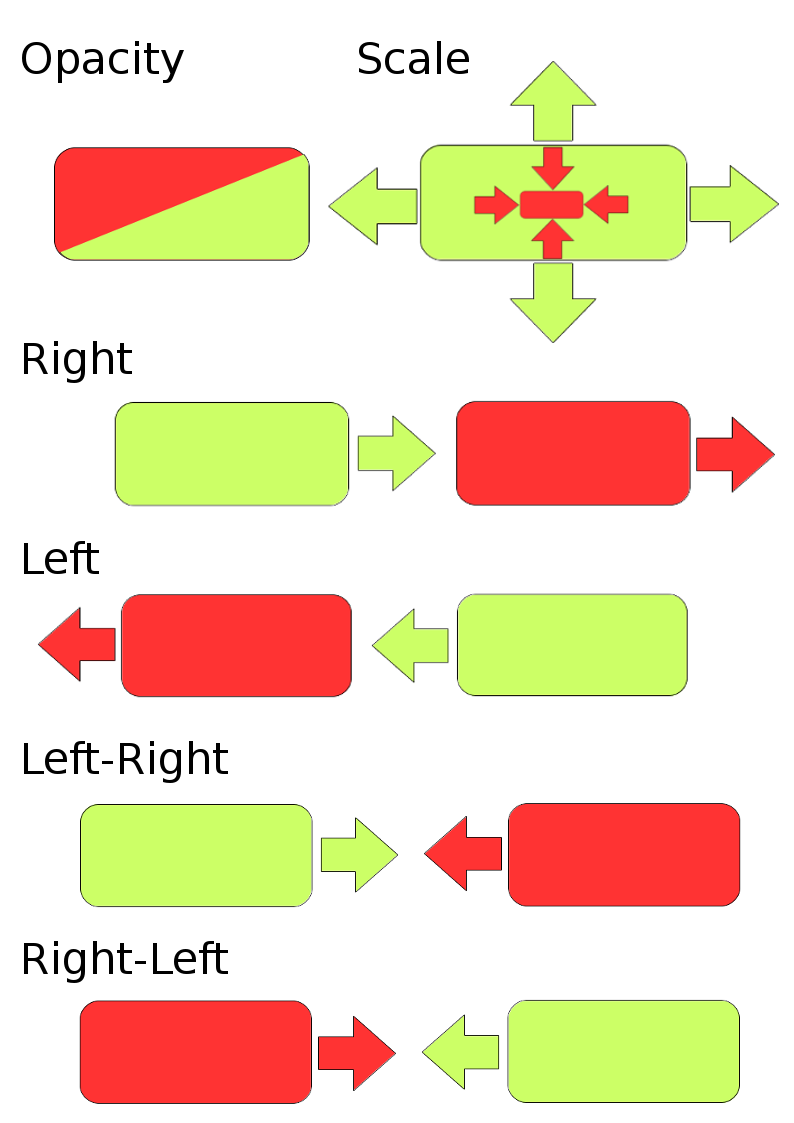
\includegraphics[width = .9\textwidth]{images/transitions.png}
	
	\caption[Slide Transition Diagram]{
		Diagram of \textit{rSlidy} included transitions and their flow. 
Red slides are the previous slides, while green are active slides. The position 
of active and previous slide is shown as relative position to the other.
		\imgcredit{Diagram is prepared by the authors of this report.}
	}
	\label{fig:transitions}
\end{figure}

% section slide_transitions (end)

\cleardoublepage
%----------------------------------------------------------------
%
%  File    :  survey-concl.tex
%
%  Author  :  Keith Andrews, IICM, TU Graz, Austria
% 
%  Created :  27 May 1993
% 
%  Changed :  16 Nov 2010
% 
%----------------------------------------------------------------


\chapter{Concluding Remarks}

\label{chap:Concl}

Through the course of further investigating web animations, we realized that 
animations are not merely there to make a website appear more beautiful, but to 
carry meaning as well. So, if a user sees a hamburger icon, they should, and 
nowadays probably they do, know what this icon stands for. We showed many other 
useful applications for animation in web UI design, how we can achieve them 
with CSS, SVG and JS. Numerous examples of code show, how powerful CSS by 
istelf can be and how each addition on top of it enhances it, which makes it 
great for RWD development 


\cleardoublepage
\printbibliography[heading=bibintoc]


\end{document}